\documentclass[a4paper,11pt]{article}

\usepackage[T1]{fontenc}
\usepackage[swedish]{babel}
\usepackage[utf8]{inputenc}

\usepackage{url}
\usepackage{graphicx}
\usepackage{geometry}
\usepackage{footnote}
\usepackage{appendix}


\setcounter{tocdepth}{2}


%--- fancyhdr -------------------------
\usepackage{fancyhdr}

\lhead{mvk13: Slutrapport}
\chead{}
\rhead{SMAB}

\fancyfoot{}
\fancyfoot[RO,LE]{\thepage}

\renewcommand{\headrulewidth}{0.4pt}
\renewcommand{\footrulewidth}{0.4pt}

\setlength{\parindent}{0cm}
\setlength{\parskip}{0.2cm}


\title{Slutrapport}
\author{SMAB}


%--- Body -------------------------------------------------
\begin{document}

\pagenumbering{gobble}

%\maketitle


%-- Title ----
\begin{titlepage}
\begin{center}

\newcommand{\HRule}{\rule{\linewidth}{0.5mm}}

\pagestyle{empty}

\textsc{\Large Playhouse}

\HRule \\[0.4cm]
{\huge \bfseries Slutrapport \\[0.4cm]}
\HRule \\[1.5cm]

\begin{minipage}[t]{0.4\textwidth}
  \begin{flushleft} \large
    \textbf{Author}\\
     John \textsc{Eriksson}          \\
     Arvid \textsc{Fahlström Myrman} \\
     Jonas \textsc{Höglund}          \\
     Hannes \textsc{Leskelä}         \\
     Christian \textsc{Lidström}     \\
     Mattias \textsc{Palo}           \\
     Markus \textsc{Videll}          \\
     Tomas \textsc{Wickman}          \\
     Emil \textsc{Öhman}
  \end{flushleft}
\end{minipage}
\begin{minipage}[t]{0.4\textwidth}
  \begin{flushright} \large
    \textbf{Supervisor}\\
    Björn \textsc{Thuresson}
  \end{flushright}
\end{minipage}

\vspace{2cm}

\section*{Beskrivning}
  \begin{flushleft}
  \par
  \begingroup
  \leftskip3cm
  \rightskip\leftskip
  Playhouse är ett projekt som går ut på att göra om en byggnad till en stor
  interaktiv display där man kan visa såväl animationer som spela enklare spel
  genom ett webbgränssnitt. På så sätt kan företag uppmärksamma sina byggnader
  på ett innovativt sätt och användare får delta på ett unikt sätt.
  \par
  \endgroup
  \end{flushleft}

\vfill

{\large \today}

\end{center}
\end{titlepage}

\pagebreak
\section*{Historik}
  \begin{description}
    \item[7/2]  reviderade dokumentet för att matcha förändringar i projektets
                utveckling och förlopp.
    \item[13/2] lade till avsnitten \emph{Dokumentation} och
                \emph{Träning}, justerade formuleringar och lade till
                skisser.
    \item[3/3]  uppdaterade researchdelen genom att lägga till vad vi
                efterforskat om gif-parsers och livestreamingtjänster.
    \item[3/3]  uppdaterade research om Gif-parser, streamingtjänst samt
                räckvidd på hue-lamporna samt deras bryggor.
    \item[7/3]  utvidgade olika avsnitt.
    \item[10/3] la till länkar och redigerade demo 2 samt hue-testet. La in
                placeholder för MS 5 i april.
    \item[23/3] la till lite information om de olika streamingtjänsterna och
                deras prisplaner samt uppdaterade milstolpe 5.
    \item[22/5] förberedde sista utkastet.
  \end{description}

\pagebreak
\tableofcontents
\pagebreak

\pagenumbering{arabic}
\pagestyle{fancy}


\section{Projektbeskrivning}

  Vi ska skapa ett system för att styra färgade lampor som ska sitta i
  fönster så att byggnaden blir en enorm skärm.  Skärmen ska kunna visa
  animationer och användas för att spela spel.  Det ska gå att i ett senare
  skede koppla elektroniska instrument (exempelvis synth) så att de utöver
  att spela upp ljud också ändrar lamporna.  När skärmen är i spelläge så kan
  spelare ställa sig i en kö i ett webbgränssnitt, där de sedan eventuellt
  paras ihop med andra spelare för att kunna spela ett spel.


\section{Mål}

  Att via ett webbgränssnitt låta användare spela ett spel där spelplanens
  pixlar består av fönster på en byggnad.  Vid en högre belastning ska
  spelarna ställas i kö.  Spelplanen ska visas för användaren med hjälp av en
  videoström av byggnaden och en virtuell spelplan för att minska problem med
  tidsfördröjning av videoströmmen.  Libido ska kunna ställa in vilket spel
  som användarna kan spela samt om det istället ska visas en animation på
  husfasaden samt hur denna animation ser ut.  Vi har också som mål att man i
  framtiden kan utvidga projektet för att hantera byggnader med speciella
  former.  Under detta projekt begränsar vi oss dock till rektangulära
  fasader.


\section{Externa förutsättningar}

  \begin{itemize}
    \item Vi måste använda lampor (troligtvis Hue) som ska belysa fönstren
          inifrån.
          \begin{itemize}
            \item Kunden måste tillhandahålla hårdvara att arbeta med
          \end{itemize}
    \item Interaktiv display.
    \item Kösystem för spelare när de väntar.
    \item Videoström av byggnaden som spelklienter kan se.
  \end{itemize}


\section{Proof-of-concept}

  En demonstration av spelet tic-tac-toe demonstrerades den 29e januari i KTHs
  lokaler på en fasad med nio fönster efter önskemål från kund utav detta.
  Detta demo bekräftar att projektidén med lampor i fönster fungerar som
  tänkt.

  Ytterligare en demonstration presenterades den 6e mars där kunden fick se
  framstegen vi gjort både på front-end och indirekt även back-end. Tic-tac-
  toe demonstrerades återigen, tillsammans med animationskapaciteten och 
  konfigurationsgränssnittet där man lägger till och testar bryggor.


\section{Roller}
  Detta är den rollfördelning som vi haft under projektets gång.

  \begin{description}
    \item[Projektledare] Emil
    \item[Projektsekreterare] Markus
    \item[Kundrelationer] Arvid
    \item[Scrum Master] Emil
    \item[Product Owner] Arvid
    \item[Kvalitetssäkring] Alla
    \item[Utveckling] Alla
  \end{description}


\section{Gruppmedlemmar}

  \begin{tabular*}{\textwidth}{l @{\extracolsep{\fill}} r}
     Namn                   & E-mail           \\
     \hline
     John Eriksson          & johne2@kth.se    \\
     Arvid Fahlström Myrman & arvidfm@kth.se   \\
     Jonas Höglund          & jhoglun@kth.se   \\
     Hannes Leskelä         & hleskela@kth.se  \\
     Christian Lidström     & clid@kth.se      \\
     Mattias Palo           & mpalo@kth.se     \\
     Markus Videll          & mvidell@kth.se   \\
     Tomas Wickman          & tomaswic@kth.se  \\
     Emil Öhman             & emiloh@kth.se    \\
  \end{tabular*}


\section{Utvecklingsmetod}

  Vi har bestämt oss för att jobba enligt den agila utvecklingsmetoden Scrum
  efter att ha jämfört olika metoder gäntemot varandra och mot de
  förutsättningar som gruppen har.  Detta beslut grundar sig på jämförelsen på
  \url{http://www.nada.kth.se/~karlm/mvk/mvk09_lec3.pdf}, som vi tycker verkar
  vara en tillförlitlig källa.

  Vi har valt att använda väldigt korta sprinter för att få mer finkornig
  kontroll över vad som görs och snabbt kunna hantera problem som uppstår om
  något tar längre tid än beräknat eller blir försenat.  Gruppmedlemmarna är
  överens om att de snabbare sprinter ger ökad effektivitet i arbetet.

  Under projektets gång förkortade vi sprinterna ytterligare. Inledningsvis
  arbetade vi med veckolånga sprinter, något vi senare kortade ner ytterligare
  då vi ansåg att arbetsbördan blev för liten. Beroende på arbetsuppgifter
  arbetar vi i sprinter som är mellan 4-7 dagar långa för att få en så bra
  tid/resultat ratio som möjligt.

\section{Planering}

\subsection{Aktiviteter}

  \begin{itemize}

    \item Utveckla lampserver
      \begin{itemize}
        \item Implementera JSON-API
      \end{itemize}

    \item Utveckla spelbackend
      \begin{itemize}
        \item API för spelmoduler
        \item Implementera tic-tac-toe som spelmodul
        \item Implementera fyra-i-rad
        \item Implementera animationsmöjligheter
      \end{itemize}

    \item Utveckla spelfrontend
      \begin{itemize}
        \item Sätta upp websocket-kommunikation
      \end{itemize}

    \item Utveckla kösystem
      \begin{itemize}
        \item Motverka botar
      \end{itemize}

    \item Utvärdera
      \begin{itemize}
        \item Lampteknik (lampräckvidd mm)
        \item Möjlighet att använda GIF
        \item Design av eget filformat?
        \item Inbäddning av videoström i spelfrontend
      \end{itemize}

    \item Dokumentera
      \begin{itemize}
        \item Lampinstallation
        \item Projektets arkitektur (separat)
        \item Installation av komponenter
      \end{itemize}

  \end{itemize}


\subsection{Beroendegraf mellan komponenter}

  \begin{center}
    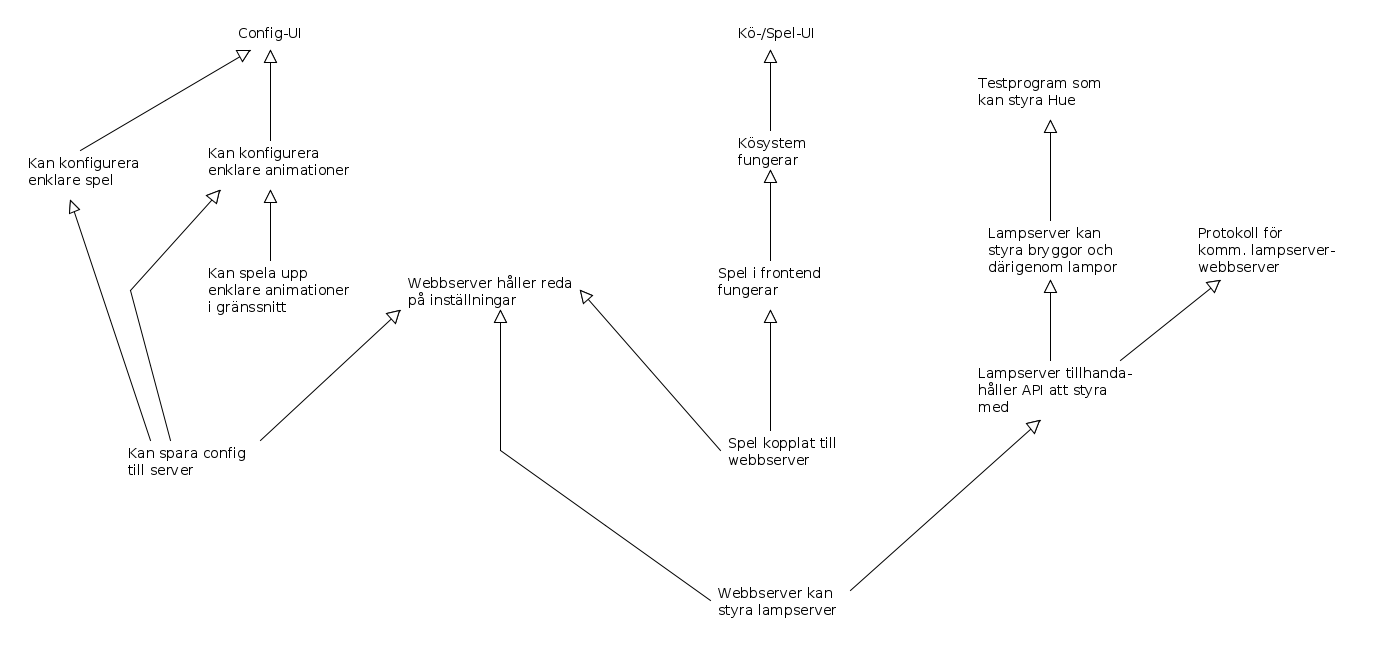
\includegraphics[width=0.9\textheight,angle=90]{task-dependencies.png}
  \end{center}
% ![Komponentberoendegraf](https://github.com/smab/meta/raw/master/deliverable/task-dependencies.png)


\subsection{Milstolpar och tidsplan}

  Milstolpar under projektets gång redovisas nedan.  Milstolparna MS1 och MS2
  har uppnåtts under tidigt skede i projektet och visas därmed ej nedan.

  \begin{itemize}
    \item MS3 (Februari 2014)
      \begin{description}
        \item[lampor] Lampserver kan styra bryggor och lampor för att ändra
                      specifika lampor.
        \item[webserver] Fungerande kösystem med turordning.
        \item[frontend] Början på UI för kösystem/spel, kösystem fungerar och
                        kopplad till server.
      \end{description}

    \item MS4 (Mars 2014)
      \begin{description}
        \item[config] Stöd för: spelkonfiguration med fyra i rad och tre i
                      rad, möjlighet att spara inställningar till server.
        \item[frontend] Fungerande spelgränssnitt, frontend klar.
      \end{description}

    \item MS5 (April 2014)
      \begin{description}
        \item[generellt] Buggfixa skriven kod
        \item[generellt] Kommentera skriven kod
      \end{description}
  \end{itemize}


\section{Forskning}

  Efter att ha utvärderat Hue-lamporna så har vi kommit fram till att dessa är
  betydligt bättre lämpade för vårt ändamål än tekniken Tellstick.  Fördelar
  med Hue-tekniken är bland annat bättre stabilitet, starkare lampor, bättre
  stöd för olika färger samt färdiga APIer som vi kan kommunicera med.  Vi har
  beslutat oss för att skriva backenden i Python, och har implementerat kod
  för att kommunicera med Hues lampservrar över HTTP via deras REST-API som
  använder JSON.

  Vi har satt upp en gemensam testplats och en testrigg med nio hue-lampor.
  Riggen är i KTHs lokaler, och vi har satt upp en kamera som streamar
  lampornas status.  Tellsticktekniken återanvänds för att kontrollera
  eltillförseln till riggen, så att lamporna kan stängas av när de inte
  används.  Lamporna kan kontrolleras utifrån, vilket gör det möjligt att
  testa ändringar utifrån.

  Vi har börjat undersöka idén att använda GIF-animationer för lagring av våra
  animationer, där tanken är att vi slipper skriva ett eget verktyg för att
  skapa animationer om det redan finns kompetenta sådana.  Istället tänker vi
  lägga större vikt på lampserverkomponenten och att få animationer att
  synkroniseras bra.  Vi har kollat på ett par olika animationsverktyg och
  konstaterat att det verkar finnas tillräckligt bra sådana tillgängliga.  En
  del tekniska bekymmer kvarstår, så som skillnaden på färgspektrum för GIF
  och våra Hue-lampor.  Vidare studier inom detta område behöver göras.

\subsection{Backend}

   När vi inledningsvis diskuterade vilka språk som vi skulle använda för de
   olika delarna i projektet så var det främst python som förespråkades.
   Då det var få av oss som hade några krav på vilket språk som skulle
   användas och några gruppmedlemmar dessutom hade goda kunskaper inom python
   så valde vi just detta för backend. Därefter påbörjade vi efterforskningar
   för att hitta ett lämpligt bibliotek för backenden, där krav låg på att
   hantera många bryggor och aktiva anslutningar.
   Tre gruppmedlemmar undersökte lika många bibliotek som vi gemensamt hade
   diskuterat fram som lämpliga: Django, CherryPy samt Tornado.

   Django bygger på designmönstret Model-View-Controller och kommer på
   förhand med diverse användbara applikationer och egenskaper. Till exempel
   så är det rekommenderat att låta Django bygga skalet för hemsidan, något
   som görs automatiskt. Därefter utvecklar man sidan i ett pythonliknande
   templatingspråk. Därtill skapas en adminkonsol som fungerar som ett sorts
   CMS, något som underlättar vid frekvent modelering av innehåll.
   Däremot tror vi inte att dessa funktioner är nödvändiga eller ens 
   lämpliga för vårt projekt.

   Det andra biblioteket som vi undersökte och till sist valde var Tornado.
   Detta beslut grundar sig på att Tornado enligt jämförelser och
   designfilosofi har som mål att klara höga belastningar samt bra inbyggt 
   stöd för tekniker så som websockets som
   vi ämnar att använda.

   Det sista alternativet vi undersökte var CherryPy. Biblioteket i sig
   var lättanvänt, till exempel så kunde man definiera flera funktioner i
   varje klass och sedan anropa dessa via URL:en /funktionsnamn. Detta i 
   motsats till Tornado där varje klass måste vara i en egen fil och man
   anropade dess klass-URL istället. Dock så hade inte CherryPy ett inbyggt
   stöd för websockets, något som gjorde att vi rankade Tornado högre.


\subsection{Räckvidd på Hue-lampor}

   För att klargöra eventuella problem i driftsatt tillstånd testade vi Hue-
   lampornas räckvidd vid olika scenarion. Detta genomfördes på KTH som har
   relativt tjocka betongväggar på ca 50 cm och likartade golv.
   Testet utgick ifrån ett script som fick lamporna tillhörande en brygga att
   blinka en gång varannan sekund i en klarblå nyans. Därefter undersökte vi
   räckvidden från brygga till lampa under följande scenarion:

   \begin{itemize}
     \item Utan hinder
     \item Antal väggar
     \item Antal golv
     \item Antal golv och väggar
   \end{itemize}

   När en lampa (A) inte fungerade testade vi också att sätta en annan lampa (B)
   mellan A och bryggan, för att på så sätt att repeater-delen fungerar bra. Med
   repeaterdelen  vill vi i framtiden också testa gruppfunktionaliteten, se så
   att man fortfarande kan få dem att blinka synkat.
   Dessvärre kunde vi inte testa lamporna genom golv mer än vad som redan 
   gjorts under demot den 29.e januari. Detta för att det inte gick att flytta 
   på bryggorna och få internetanslutning på den nya platsen. Detta berodde 
   förmodligen på att de fick en annan ip adress än den vi skickade våra 
   meddelanden till, något som kanske berodde på KTH:s nätverksstruktur.

   Resultatet av de övriga testerna var någorlunda hoppfulla för vårt ändamål.
   Sedan tidigare visst vi att bryggan klarar av att skicka sina signaler genom
   KTH:s golv. Även genom en vägg fungerade väl, men vi märkte direkt att
   ytterligare obstruktion gjorde att signalerna förlorades antingen periodvis
   eller fullständigt.
   Därefter fortsatte vi genom att testa repeatereffekten hos hue-lamporna. 
   Utan hinder så kunde vi konstatera att varje lampa kunde skicka signalen
   cirka 20 meter utan att några fördröjningar uppstod. Längre än så kunde man
   inte garantera synkroniserat blinkande.
   Därefter fortsatte vi genom att testa hue-lampornas repeatereffekt genom
   väggar.

   Det som kvarstår att testa är således hur många lampor man kan seriekoppla 
   och eventuella delays som ett resultat av detta, samt att seriekoppla genom 
   golv.

\subsection{Gif-parser}

   För att hantera skapandet av animationer har vi valt att skapa gif-bilder
   vid varje animationssteg för att sedan tolka dessa på ett sätt som
   lamporna kan förstå. Det huvudsakliga resultatet ifrån denna efterforskning
   ledde till användandet av pythonbiblioteket Pillow, en fork av PIL, som har
   väl definierade metoder att nyttja för att implementera de funktioner
   vi behöver.

   Våra krav på biblioteket var möjlighet att kunna:

   \begin{itemize}
     \item Läsa in en bild
     \item Byta frame
     \item Läsa in längd av en frame
     \item Observera en enskild pixel
     \item Hämta information från enskild pixel
   \end{itemize}

   Andra bibliotek som undersöktes var:

   \begin{itemize}
     \item Mahotas
     \item Scikit-Image
     \item Insight Segmentation and Registration Toolkit(ltk) 
     \item OpenCV
     \item Medical image processing in Python (MedPy)
   \end{itemize}

   Då Pillow hade allt vi behövde och var enkelt att implementera blev det
   ingen större debatt kring valet av bibliotek, utan vi implementerade en 
   gif-parser med hjälp av detta bibliotek.


\subsection{Stream-tjänster}

  Vi har arbetat med idén att använda GIF-animationer för lagring av våra
  animationer, där tanken är att vi slipper skriva ett eget verktyg för att
  skapa animationer då det redan finns kompetenta sådana som vi funnit efter 
  en del efterforskningar.  Istället tänker vi lägga större vikt på 
  lampserverkomponenten och att få animationer att synkroniseras bra.  Vi har
  kollat på ett par olika animationsverktyg och konstaterat att det verkar
  finnas tillräckligt bra sådana tillgängliga. En del tekniska bekymmer 
  kvarstår, så som skillnaden på färgspektrum för GIF och våra Hue-lampor.
  Vi har hittat gif-verktyg som verkar passa våra behov bra. Då det enda vi
  egenligen eftersöker är ett enkelt gränssnitt för att skapa simpla 
  animationer så spelar det inte så stor roll om det saknar en del 
  funktionalitet. Likt livstreamingtjänsen så kommer det i slutändan inte 
  vara vi som kommer behöva tilhandahålla ett gifanimeringsverktyg utan vi 
  ska bara tillföra möjligheten att kunna ladda upp gifanimationer till 
  servern så att denna spelar upp animationen till lamporna. Vi har dock 
  genomfört en del forskning inom verktyg och kommit fram till att Asesprite 
  verkar som ett lämpligt verktyg för att utföra de tester som vi behöver 
  utföra. Det är dessutom släppt med öppen källkod på programmet vilket vi 
  tycker är ett plus.

  Vi har diskuterat olika livestreamingtjänster inom gruppen som verkar 
  lämpliga, men det är svårt att dra några slutsater i detta skede då det 
  ligger utanför våran arbetsbeskrivning att implementera en streamingtjänst.
  Men att på ett enkelt sätt tillhandahålla möjligheten att implementera en 
  livestreaming på våran hemsida känns som en relevant och överkomlig uppgift.

  De livestreamingtjänster och program för inspelning som vi diskuterat inom 
  gruppen är som följer med sin för/nackdelar:

  \begin{itemize}
    \item XSplit
      \begin{itemize}
        \item Betallösning
        \item Endast Windows
      \end{itemize}

    \item OBS (Open Broadcaster Sowftware)
      \begin{itemize}
        \item Gratis
        \item Windows, Linux kommer släppas
      \end{itemize}

    \item FFSplit
      \begin{itemize}
        \item Gratis
        \item Windows
      \end{itemize}

    \item Wirecast
      \begin{itemize}
        \item Betallösning
        \item Windows, Macintosh
      \end{itemize}

    \item FFmpeg
      \begin{itemize}
        \item Gratis
        \item Windows, Macintosh, Linux
        \item Kommandorad
        \item Massa bra info, bla om tidsfördröjning och hur man kopplar ihop
              med twitch.  \url{https://trac.ffmpeg.org/wiki/StreamingGuide}
      \end{itemize}

    \item Simple Screen Recorder
      \begin{itemize}
        \item Gratis
        \item http://www.maartenbaert.be/simplescreenrecorder/live-streaming/
        \item Kommandorad, och vanligt
        \item Kan vara buggigt
      \end{itemize}
  \end{itemize}

Följande företag tillhandahåller streamingtjänster

  \begin{itemize}
    \item Livestream
      \begin{itemize}
      \item Gratis men med möjlighet att betala för mer tjänster.  Dessa
            verkar dock mest ha att göra med att man far tillgång till deras
            videoredigeringsverktyg
      \item \url{http://new.livestream.com/plans}
      \end{itemize}

    \item Bambuser
      \begin{itemize}
      \item Har gratis alternativ som inte är ett alternativ för våran applikation
      \item Kostnaden hänger ihop med hur många tittartimmar som man vill köpa
            och överstiger man dessa timmar sa kostar det extra per timma
      \item http://bambuser.com/premium
      \end{itemize}

    \item Ustream
      \begin{itemize}
      \item Gratisalternativ för privatpersoner
      \item Baserar sig ocksa på tittartimmar
      \item För deras 'Enterprise' prisplan får man kontakta dem
      \item \url{https://www.ustream.tv/platform/plans#itm_source=footer&itm_medium=plans_pricing_link&itm_content=Plans_and_Pricing&itm_campaign=footer}
      \end{itemize}

    \item Justin.tv
      \begin{itemize}
      \item Baserar sig på tittartimmar
      \item även dessa har ett enterprisealternativ
      \item \url{http://www.justin.tv/payments/premium/}
      \end{itemize}

    \item Twitch
      \begin{itemize}
      \item Verkar rätt nischat på spel
      \item Har ingen riktig betalplan men man kan bli 'twitch partner' för diverse fördelar
      \item \url{http://www.twitch.tv/p/partnersvideo}
      \end{itemize}
  \end{itemize}


\section{Scenarier, krav och behov}

  Detta avsnitt beskriver de scenarier, krav och behov som vi satt upp som
  stöd under projektets gång.

\subsection{Scenarier}

\subsubsection*{Scenario 1: byggnadsägare}

  Glenn ska inviga en byggnad i centrala Göteborg och vill ha något spektakulärt.
  Han bestämmer sig för att anlita Libido Music för att installera lampor och
  göra någon cool show. Libido kommer och installerar lampor i Glenns byggnad
  samt gör en demo. Showen görs av Libido hos deras kontor vid Karlaplan och
  visas på något sätt upp på invigningsdagen.

\subsubsection*{Scenario 2: slutkund}
  Karl-Bertil går förbi en cool byggnad i stan med massa lampor på. Han ser en
  liten informationsskylt framför byggnaden som säger att om han går in på
  example.com så kan han spela ett spel där han använder byggnaden som en stor
  skärm. Han skriver in addressen och hamnar i en kö. Det står att han har plats
  10 av 11.  Till slut kommer han att paras ihop med någon annan spelare och de
  kan på ett enkelt sätt spela något spel.


\subsection{Krav}

  Användaren måste kunna

  \begin{itemize}
    \item Skapa en animation
      \begin{itemize}
        \item Tänder lampor i olika färger och styrkor
        \item Sätta färg, styrka, tidsfördröjning på lampor.
      \end{itemize}

    \item Spela enkla spel
      \begin{itemize}
        \item Minst ett spel. Tic-tac-toe, 4-i-rad...
        \item Mot varandra
        \item Spelare hamnar i en kö
      \end{itemize}

    \item Libido/byggnadsägaren ska ha möjlighet att enkelt administrera
          installationen.
      \begin{itemize}
        \item Byta spel samt konfigurera färgval
        \item Byta animation
        \item Skärmsläckare (dvs animation) om ingen spelar?
      \end{itemize}
  \end{itemize}

  Se även tidigare avsnitt om projektets externa förutsättningar.


\subsection{Extrafunktionalitet}
  Detta är funktioner som vi implementerade i mån av tid.  Vi har inte
  implementerat något stöd för ickerektangulära fasader, men däremot är
  funktionen för hopkopplingen mellan lampor och bryggor implementerad så att
  det är enklare att installlera Playhouse i en ny byggnad.

  \begin{itemize}
    \item Stöd för olika form på fasader

          I dagsläget förutsätter vi rektangulära husfasader, men i praktiken kan
          många aktuella hus ha ickerektangulär fasad.  I sådana fall är det
          önskvärt att på något sätt kunna ange utseendet på fasaden.

    \item Förenkla hopkoppling mellan lampor och bryggor

          Idag behöver man koppla samman lampor med bryggor genom att skruva i en
          i taget och köra ett program mellan varje lampa.  Det skulle förenkla
          installation av lampor i byggnad avsevärt om man kunde skruva i alla
          lampor på en gång och sedan via ett gränssnitt mappa lamporna till
          pixlar.

          För att verifiera att allt satts upp i rätt ordning vore det användbart
          med ett testprogram som lyser upp lamporna enligt ett förbestämt
          mönster, ex. rad för rad och kolumn för kolumn.
  \end{itemize}


\section{Teknologi och arkitektur}

  Vår applikation har två sorters användare: dels vår klient, som behöver kunna
  skapa animationer etc., och dels vanliga personer som ansluter via en
  webbläsare för att spela. För att kunna hantera flera spelare implementerar vi
  ett kösystem, då det inte går att spela flera spelomgångar samtidigt. När en
  spelare har nått längst fram i kön kommer spelaren att få se något gränssnitt
  där den kan spela själva spelet samt livevideo som visar den faktiska
  byggnaden där lamporna är installerade.

  Detta innebär att det behövs någon sorts webbserver som har som funktion att
  skicka individuella sidor till användaren, samt som hanterar kö- och
  spellogiken. Vi har bestämt oss för att använda Python tillsammans med
  webbservermjukvaran Tornado, se diskussion under Research tidigare i
  dokumentet.

  Vi behöver också någon komponent så hanterar kommunikation med de bryggor som
  i sin tur kommunicerar direkt med lamporna. Vi ansåg att det vore lämpligt att
  implementera webbkomponenten och lampkommunikationskomponenten som två
  separata servrar.

  Då vi behöver kunna visa livevideo från byggnaden kommer vi också att behöva
  kunna kommunicera med någon server som är kopplad till en kamera.  Detta är
  tänkt att ske via en streamingtjänst, exempelvis Bambuser.


\subsection{Arkitekturdiagram}

  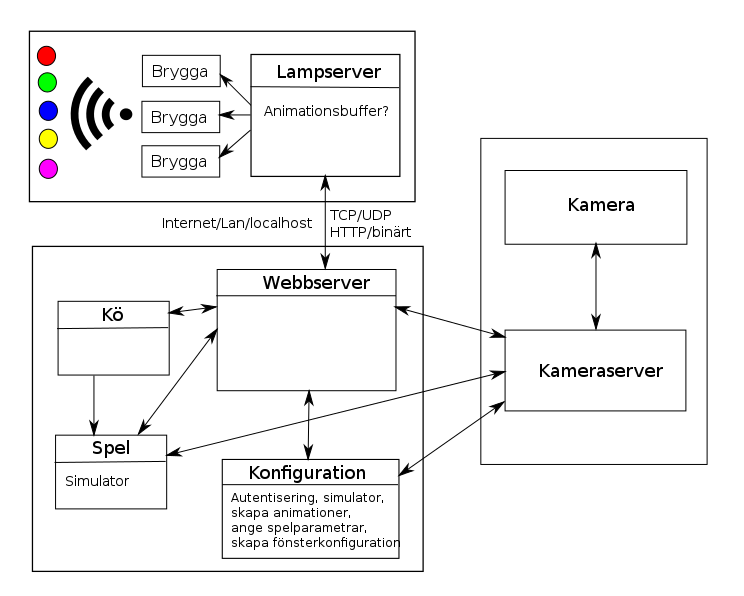
\includegraphics[width=\textwidth]{component_diagram.png}

% ![Komponentdiagram](https://github.com/smab/meta/raw/master/deliverable/component_diagram.png)
% ![Motsvarande i .svg-format](https://docs.google.com/file/d/0B4acd1MFyToeSkdFRmhEdWFGSkE/edit?pli=1)


\section{Risker}

  Nedan följer de risker vi har förhållit oss till i projektet.
  De flesta av riskerna har vi till stor del lyckats undvika,
  då de antingen varit lätta att lösa eller helt enkelt inte inträffat.

  Några få av riskerna ligger dock fortfarande i framtiden, då vi ännu
  inte haft chans att testa projektet i stor skala som vi skulle önska.
  Några exempel på detta skulle kunna vara att servern överbelastas,
  eller att webbkamerastreamingen av huset syns dåligt. Dessa risker
  bör dock vara utanför vårt ansvarsområde.

  \begin{savenotes}
  \begin{tabular}{p{0.4\textwidth} p{0.4\textwidth} l l}

    {\bf Risk} & {\bf Åtgärd} & {\bf Sann.} & {\bf Impact} \\
    \hline
     Kommunikation mellan bryggor och lampor är opålitlig (väldigt stor
     fördröjning, tappar signaler, etc.) &
     Fixa eventuella buggar; Använda fler bryggor vid behov; Programmera egen
     brygga &
     Hög &
     Hög \\
     \hline

     Kommunikation mellan lampservern och bryggorna är bristfällig (för
     långsam/opålitlig) &
     Fixa eventuella buggar; Fixa diverse tekniska problem med anslutning &
     Medel &
     Hög \\
     \hline

     Lamporna stör varandra när de har olika färger (t.ex. två fönster inom
     samma rum) &
     Skärmar mellan lamporna; Begränsa så att lampor i samma rum alltid har
     samma färg &
     Låg &
     Medel \\
     \hline

     Problem med ihopkopplingen av delsystem(lamp- och webbserver etc.)
     (interna protokoll matchar inte, inkorrekt data, etc.) &
     Fixa eventuella buggar &
     Medel &
     11/10 \\
     \hline

     Webbservern och/eller webbgränssnittet är instabila &
     Fixa eventuella buggar &
     Medel &
     Medel \\
     \hline

     Webbservern får fler besökare än den kan hantera (överbelastning, stort
     intressen, DoS) &
     Köra webbserver i molnet (Amazon eller liknande); Optimera koden lite;
     Stäng av spel och spela animation istället (ej interaktiv dock);
     Iptables-magi? (droppa paket) &
     Låg &
     Medel \\
     \hline

     Osynkade animationer (lampor byter färg i varierande hastigheter så att
     lamporna är i osynk med varandra) &
     Använda fler bryggor; Begränsa animationerna så att de inte är för
     beroende av perfekt synk &
     Medel &
     Medel \\
     \hline

     Webbkamerastreaming fungerar dåligt (lamporna syns dåligt, dålig
     bildkvalitet, laggigt, ingen bild alls, kameran ramlar ner) &
     Fixa eventuella buggar; Bättre Internetuppkoppling; Bättre kamera; Bättre
     kamerainstallation &
     Medel &
     Medel \\
     \hline

     Huset syns dåligt i webbkameran p.g.a väderleksförhållanden eller
     liknande, t.ex. regn eller dimma. &
     Bättre väder\footnote{\url{http://en.wikipedia.org/wiki/Weather_modification}};
     Stänga av Playhouse när det är dålig sikt &
     Låg &
     Låg \\
     \hline

  \end{tabular}
  \end{savenotes}

\newpage
\section{Dokumentation och träning}

\subsection*{Dokumentation}
  Dokumentation av kodbasen görs successivt under utvecklingen, så att
  framtida utvecklare kan ta över och fortsätta projektet.  Själva
  arkitekturen och installation av komponenter måste också dokumenteras.
  Dokumentation av arkitekturen finns i begränsad mån i detta dokument i
  dagsläget, men bör migreras till ett separat dokument och göras mer
  fullständig.

\subsection*{Träning}
  Vårt projekt involverar två sorters användare: de som installerar lamporna
  och bestämmer vad som visas, och slutanvändare som interagerar med
  installationen genom spel via en spelfrontend.  Det senare är
  förhoppningsvis intuitivt (spelarna antas känna till reglerna för tre-i-rad
  och fyra-i-rad).  Den förstnämnda gruppen behöver dock någon form av guide,
  inte minst för installationen av lampor.  Det nuvarande systemet för
  installation är temporärt; vi planerar att dokumentera uppsättningsprocessen
  när vi har fått ett bättre system på plats.  Även hur man ställer in
  animation och väljer spel bör dokumenteras, men för detta ändamål bör det
  räcka med en relativt kort hjälptext i själva gränssnittet.


\begin{appendices}
\newpage
\section{Skisser}

  I detta appendix inkluderas skisser på de olika gränssnitt olika typer av
  användare kan se, som berör projektet.

\subsection{Konfiguration}
  Vår idé kring hur konfigurationsgränssnittet kunde se ut inkluderas nedan.

  \begin{center}
    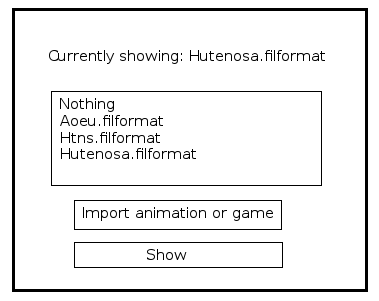
\includegraphics[width=0.4\textwidth]{images/sketch-config.png}
  \end{center}
% ![Konfiguration](https://github.com/smab/meta/raw/master/deliverable/images/sketch-config.png)

  Det nuvarande konfigurationsgränssnittet:

  \begin{center}
    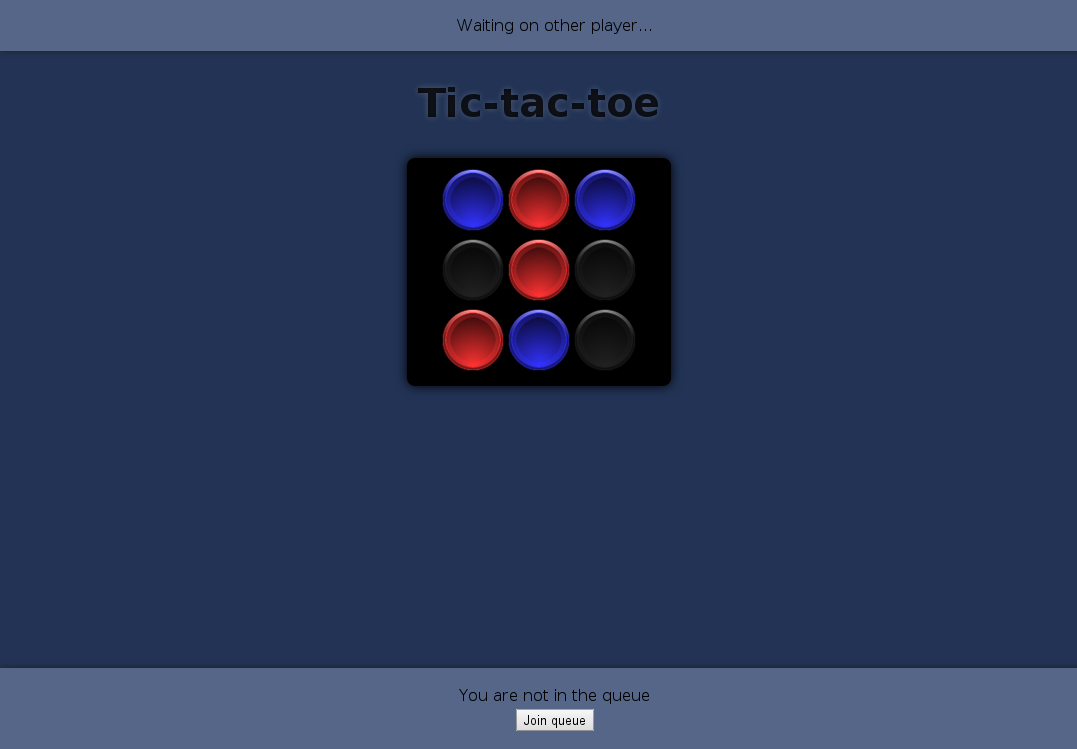
\includegraphics[width=0.9\textwidth]{sepdata1.png}
  \end{center}
% ![Konfiguration](https://github.com/smab/meta/blob/master/deliverable/sepdata1.png)

  Vi avvek alltså ganska mycket från ursprungsidén, framför allt eftersom vi
  tog beslutet att helt enkelt representera animationer som GIF-bilder
  istället för ett eget filformat.

\subsection{Spel}
  Vi hade tidigare flera idéer på hur spelgränssnittet kan se ut.  Skisser på
  designidéer inkluderas nedan.

  \begin{center}
    \begin{tabular}{c c}
      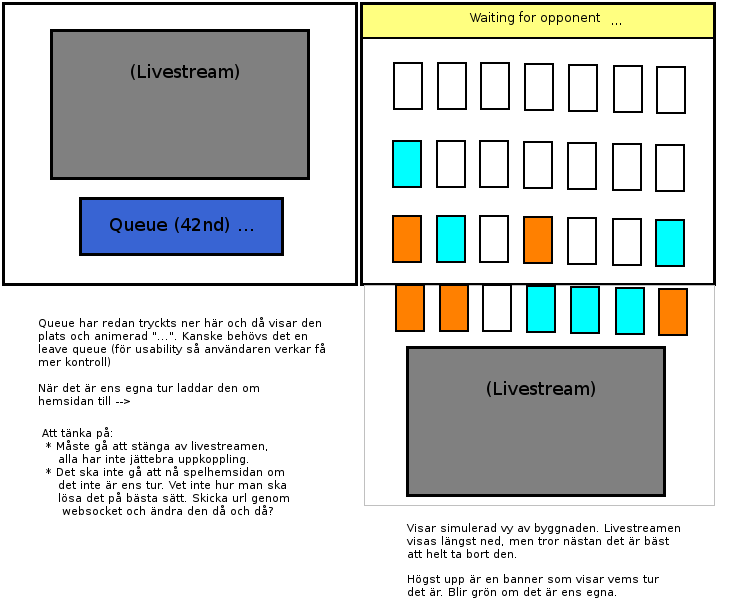
\includegraphics[width=0.5\textwidth]{images/sketch-game-1.png}
      &
      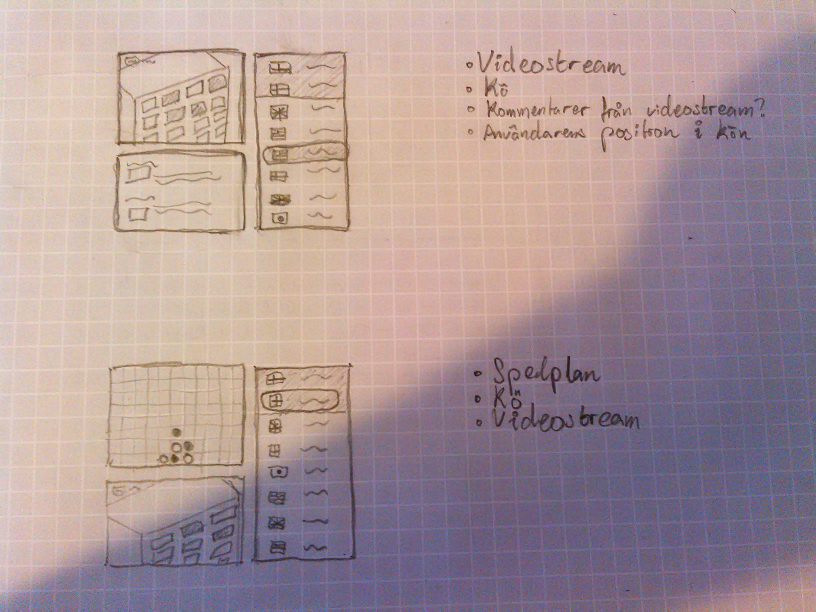
\includegraphics[width=0.5\textwidth]{images/sketch-game-2.jpg}
    \end{tabular}
  \end{center}

% ![Spelfrontend: förslag 1](https://github.com/smab/meta/raw/master/deliverable/images/sketch-game-1.png)

% ![Spelfrontend: förslag 2](https://github.com/smab/meta/raw/master/deliverable/images/sketch-game-2.jpg)

  Det nuvarande spelgränssnittet:

  \begin{center}
    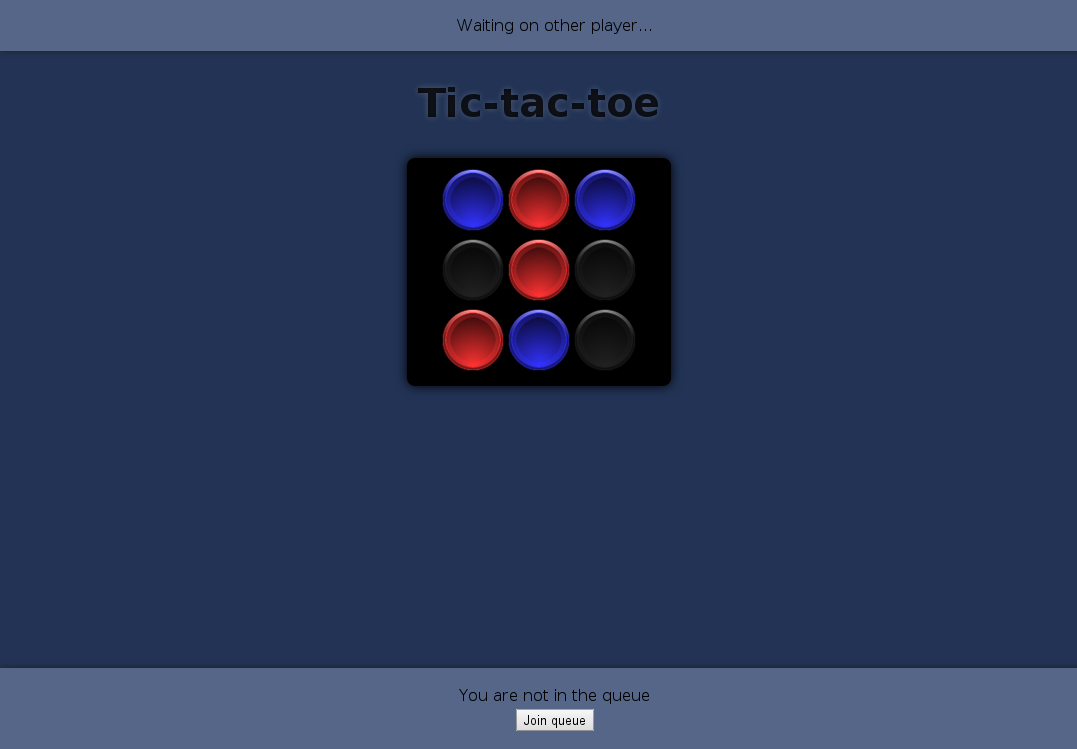
\includegraphics[width=0.8\textwidth]{sepdata2.png}
  \end{center}

% ![Spelfrontend: aktuella](https://github.com/smab/meta/blob/master/deliverable/sepdata2.png)




\newpage
\section{Dokumentation: konfiguration}
  Detta appendix innehåller dokumentation kring konfigurationen av en
  installation av Playhouse.  Kapitlet är på engelska eftersom källkoden till
  projektet ligger öppet allmänheten och dokumentationen då ska nå ut till så
  många som möjlight som är intresserade av projektet.

  Se \url{https://github.com/smab/playhouse-web/wiki/Configuration} för
  senaste versionen av detta appendix.


\subsection{Overview}
The configuration interface can be reach as a webpage on
\url{http://localhost:<config_port>/config} where the default port is 8081.

There are six source files directly associated with this module, which can be
found in the relevant directories:

  \begin{description}
    \item[config.py]
     the main module source code, responsible for handling all requests in the configuration interface
    \item[config\_base.html]
     base template file
    \item[config\_setup.html]
     template file for Setup
    \item[config\_game.html]
     template file for Settings
    \item[config\_bridges.html]
     template file for Bridges
  \end{description}

\subsection{Configuration file}
Everything under Setup and Settings can also be changed manually in
\texttt{config.json}.

\subsubsection{Attributes}
  \begin{description}
    \item[\texttt{game\_name}:] name of initial game module to start (default: \texttt{"default"})
    \item[\texttt{game\_path}:] list of paths to where games can be found (default: \texttt{["src/games"]})
    \item[\texttt{lampdest}:] address to lamp server (default: \texttt{"localhost"})
    \item[\texttt{lampport}:] port to connect to lamp server (default: \texttt{4711})
    \item[\texttt{serverport}:] port the game server will listen on (default: \texttt{8080})
    \item[\texttt{configport}:] port the config server will listen on (default: \texttt{8081})
    \item[\texttt{stream\_embedcode}:] HTML string with stream embed code (default: \texttt{""})
    \item[\texttt{light\_ssl}:] set to \texttt{true} to connect to the lamp server with HTTPS
    \item[\texttt{light\_certfile}:] only needed if \texttt{light\_ssl} is \texttt{true}
    \item[\texttt{light\_pwd}:] password used to authorize with the lamp server
    \item[\texttt{config\_ssl}:] when \texttt{true}, run config interface on a HTTPS server
    \item[\texttt{config\_certfile}:] only needed if \texttt{config\_ssl} is \texttt{true}
    \item[\texttt{config\_keyfile}:] only needed if \texttt{config\_ssl} is \texttt{true}
    \item[\texttt{config\_pwd}:] when set, password needed to access config
  \end{description}

\subsection{Configuration interface}
\subsubsection{Setup}

This page contains settings for connections and external services.
Some of settings may require that the server is restarted.

\subsubsection{Connections}

  \begin{description}

    \item[Status]
        Show the current connection status to the lamp server.
    \item[Lamp server]
        Address to the lamp server and what port to connect to. (default:
        \texttt{localhost:4711})
    \item[Game server port]
        This is the port the web server that serves the game interface will
        listen on. (default: \texttt{8080})
    \item[Config server port]
        This is the port the web server that serves the configuration
        interface will listen on. (default: \texttt{8081})

  \end{description}

  Note: Do not use the same port for game and config or the game interface
  will not be able to start.

\subsection{Streaming}
  \begin{description}
    \item[Embed code]
        The content in this text area will be inserted in the game interface
        and is primarily for embedding a live stream player. (default:
        \textit{empty})
  \end{description}


\subsubsection{Settings}
This pages is used to change game and game settings.

\subsubsection{Changing game}
All games found in the game paths is listed to the left and the current game
can be changed directly by clicking on any of the listed games.  Note:
Changing game paths has to be done by editing \texttt{game\_paths} in the
config file.

\subsubsection{Game settings}
Game settings are shown on the right and will show the config template
specified by \texttt{config\_file} in the the running game module. For more
information, see the documentation on game settings for each module.


\subsection{Bridges}
This menu handles all the Hue bridges that are used. It lists all bridges the
lightserver knows about, sorted by their MAC-address.

\subsubsection{Identifying Selected}
By selecting bridges with the checkbox, you can tell the bridge to blink all
the lamps associated with this bridge by pressing the "Identify Selected"
button.

\subsubsection{Valid username}
Each Hue bridge needs a username. This acts like a password so unauthorized
people cannot send commands to your lamps. Each bridge in the table has a
property \texttt{valid\_username} which tells you if the lightserver knows about a
valid username for that bridge. By clicking the property, you can tell the
lightserver to generate a new username. A confirmation box will appear and you
will have to physically  press the link button on the bridge before accepting.

\subsubsection{Adding bridges}
You can add a new bridge by writing its IP address in the textfield and
pressing ``Add bridge.''

\subsubsection{Removing bridges}
You can remove bridges by select them with the checkboxes and then pressing
``Remove Selected.''

\subsubsection{Refresh List}
A cached copy of the bridges will be saved on the webserver to decrease
waiting time. If any changes happens to the bridges it will not be shown
however. You can force a request for a new version by pressing the ``Refresh
List'' button.

\subsubsection{Search Bridges}
If you know there are bridges on the same local network as the lightserver,
you can have it search for them. It will do that by a broadcast message and by
reading the Philips website. This search may take some time though and after
about 20s you \textit{must} refresh the list by pressing the ``Refresh List''
button.


\subsection{Grid}

This page is used to configure the lamp positions in the grid and the
dimensions of the grid.  The grid overview shows the positions where lamps are
placed and the status of those lamps.

\subsubsection{Color coding (interface)}
  \begin{description}
    \item[white] no lamp placed
    \item[blue]  a lamp is placed here and no errors found (note: the lamp
                 server can't know if a lamp is reachable or not)
    \item[red]   a lamp is placed here but there is no bridge with this lamp id
  \end{description}

\subsubsection{Color coding (lamps)}
  \begin{description}
    \item[white] activated lamp
    \item[blue]  placed lamp
    \item[red]   removed lamp
  \end{description}

\subsubsection{Placing lamps}
Before placing the lamps, it is recommended to first turn off any running
games. It can be done directly from the grid page by clicking on the ``Turn
Off'' button.

When you open the page, a lamp light up and then can you say which lamp was
lit. This can be done either by clicking on the overview or manually enter the
position and then click on ``Place Lamp''. Attempting to place a lamp on an
occupied position will instead remove the currently placed lamp on that
position and queue it for placement.

\subsubsection{Changing size}
Changing size is done by entering the dimensions as \texttt{widthxheight} and then
click ``Change Size''.  Note: This will clear the grid and because of that the
``Change Size''-button will be disabled to prevent loss of unsaved changes.
Saving or refreshing will reenable the button.

\subsubsection{Actions}
  \begin{description}
    \item[Save]             Send and use the grid on the lamp server.
    \item[Refresh]          Discard the local grid and request the one currently used on the lamp server.
    \item[Clear]            Clear the grid from placed lamps.
    \item[Turn Off]         Cancel any running game and turn off all lamps.
    \item[Run Diagnostics]  Run diagnosics to test the grid on the lamp server.
  \end{description}

\subsubsection{Errors}
  \begin{description}
    \item[No activated lamp]  there is either no more lamps available that isn't already placed
    \item[Invalid position]   the position were in an incorrect format and couldn't be parsed be the server
    \item[Invalid size]       the size were in an incorrect format and couldn't be parsed be the server
    \item[Invalid lamp]       the placed lamp is no longer valid and can't be placed
    \item[Saving failed]      given when the lamp server couldn't save the grid
  \end{description}

\end{appendices}

\end{document}
